\documentclass[11pt]{amsart}
\usepackage{geometry}                % See geometry.pdf to learn the layout options. There are lots.
\geometry{letterpaper}                   % ... or a4paper or a5paper or ... 
%\geometry{landscape}                % Activate for for rotated page geometry
%\usepackage[parfill]{parskip}    % Activate to begin paragraphs with an empty line rather than an indent
\usepackage{graphicx}
\usepackage{amssymb}
\usepackage{epstopdf}
\usepackage[usenames,dvipsnames]{color}
\usepackage{fancyvrb}
\usepackage{listings}
\usepackage{booktabs,footmisc}
\usepackage{hyperref}
\usepackage[all]{hypcap}

\usepackage{topcapt}
\usepackage{enumerate}
\usepackage[section] {placeins}

 
% include the lines below to use a nicer fixed-width font than the default one
 
\lstset{fancyvrb=true}
\lstset{
	basicstyle=\small\tt,
	identifierstyle=,
	commentstyle=\color{Bittersweet},
	stringstyle=\color{red},
	showstringspaces=false,
	tabsize=3,
	numbers=left,
	captionpos=b,
	xleftmargin=2em
%	numberstyle=\tiny
	%stepnumber=4
	}
\DeclareGraphicsRule{.tif}{png}{.png}{`convert #1 `dirname #1`/`basename #1 .tif`.png}

\title{Repast Parameter Sweeps Getting Started}
\author{Mark Bragen \& Mark Altaweel}
%\date{\today}                                           % Activate to display a given date or no date

\begin{document} 
\maketitle

\section{Parameter Sweeps}
The Repast Simphony User Interface has been extended to provide a mechanism for creating parameter sweep and optimized sweep definition files. These definition files can then be submitted for execution in either a distributed grid environment or on the local computer. Fig.~\ref{fig:sweep1}  is a screen capture of the Parameter Sweep window for the Predator Prey Model.\\

\begin{figure}[h]
\begin{center}
\vspace{.2in}
\centerline {
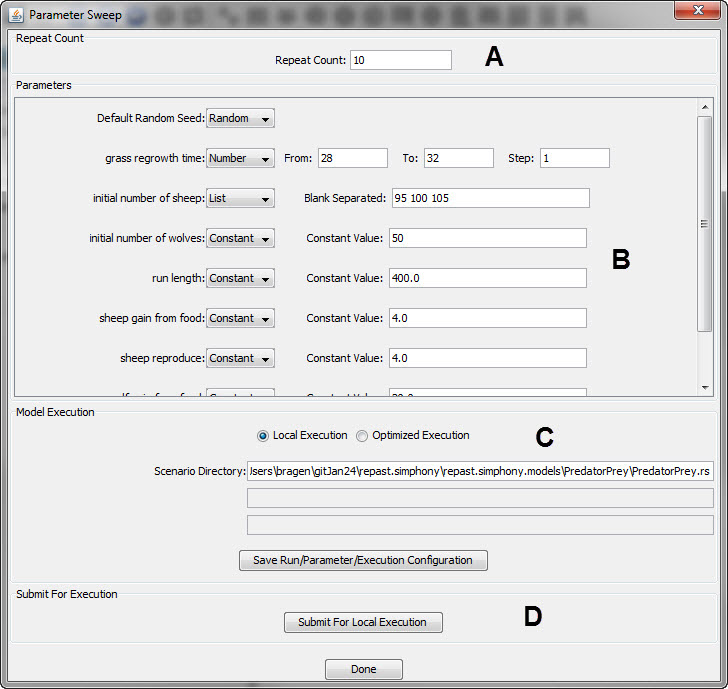
\includegraphics{images/Sweep1.jpg}
}
\caption{}
\label{fig:sweep1}
\end{center}
\end{figure}

The window is divided into four sections:
\begin{enumerate}[ (A) ]
\item Specify the repeat count for the sweep
\item Specify the parameter value definitions for a single sweep
\item Specify the require file information based on execution mode
\item Run submission
\end{enumerate}
\vspace{.2in}

In Section A (see Fig. ~\ref{fig:sweep2} ), the user specifies the number of times that the parameter sweep definitions from Section B will be executed. Note that the parameter sweep definition in Section B specifies a single unit of work that will be executed (i.e. multiple model executions with varying parameter values).\\

\begin{figure}[h]
\begin{center}
\vspace{.2in}
\centerline {
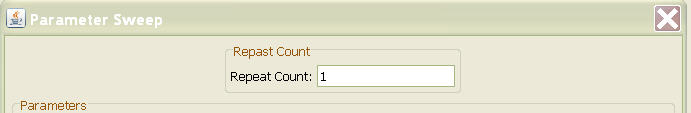
\includegraphics{images/sweep2.jpg}
}
\caption{}
\label{fig:sweep2}
\end{center}
\end{figure}

In Section B (Fig. ~\ref{fig:sweep3}), the user specifies the values for each of the model parameters. Except for the Default Random Seed value, the value(s) can be specified in one of three ways:

\begin{enumerate}
\item A constant value 
\item A list of blank separated values
\item A list of values specified with from, to, step definition
\end{enumerate}
\vspace{.2in}

\begin{figure}[h]
\begin{center}
\vspace{.2in}
\centerline {
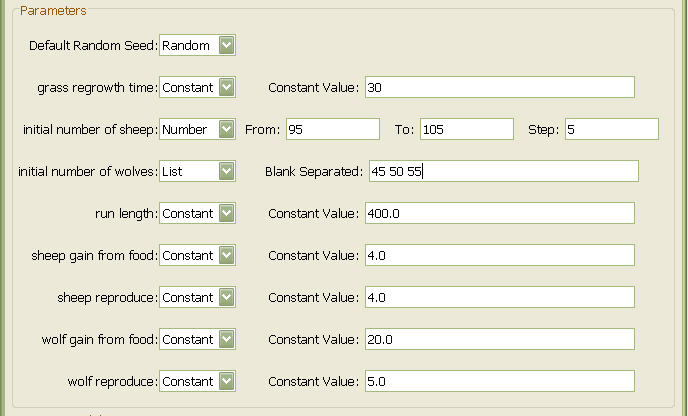
\includegraphics{images/sweep3.jpg}
}
\caption{}
\label{fig:sweep3}
\end{center}
\end{figure}


These are selected from the drop-down selection. Values must be specified for all model parameters. The Default Random Seed has an additional option of a completely random specification. The Random Seed will be determined during the execution of the model.\\

In Section C, the user specifies the type of execution. Three types, each of which has different information requirements, are available:
\begin{enumerate}
\item Local Execution � Execution of the model on the local machine
\item Optimized Execution � Execution of the model on the local machine using a specified optimizer
\item Grid Execution � Execution of the model across GridGain nodes.
\end{enumerate}
\vspace{.2in}

In Local Execution mode, the user simply needs to specify the Scenario Directory (see Fig. ~\ref{fig:sweep4a}). Note that this text field is filled by using the scenario directory provided as an argument to the launcher. 

\begin{figure}[h]
\begin{center}
\vspace{.2in}
\centerline {
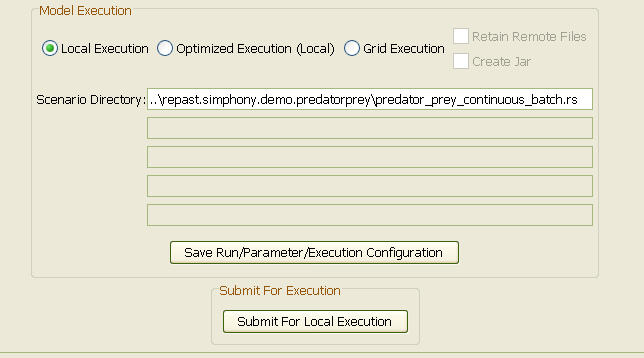
\includegraphics{images/sweep4a.jpg}
}
\caption{}
\label{fig:sweep4a}
\end{center}
\end{figure}

In Optimized Execution mode, the user must specify the Run Result Producer and the Advancement Chooser in addition to the Scenario Directory (see Fig. ~\ref{fig:sweep4b}). Please reference the definitions of these two items in the batch processing documentation. 

\begin{figure}[h]
\begin{center}
\vspace{.2in}
\centerline {
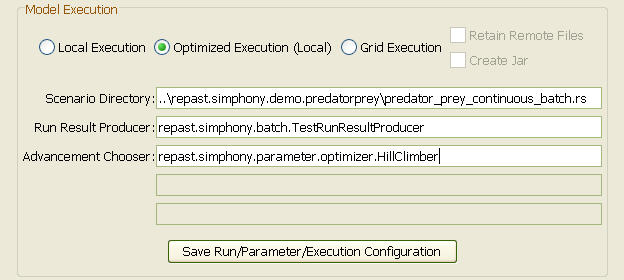
\includegraphics{images/sweep4b.jpg}
}
\caption{}
\label{fig:sweep4b}
\end{center}
\end{figure}

In order to use Grid Execution mode, the user must download and install the GridGain software package and complete the GridGain and Repast Simphony Grid Extension installation procedure as documented below. If GridGain is installed, the Model Execution portion of the window will appear as in Fig. ~\ref{fig:sweep4c} where the �Grid Execution� radio button and the two check boxes are enabled. If GridGain is not installed, the Model Execution portion of the window will appear as in Fig. ~\ref{fig:sweep4d} where the radio button and check boxes are disabled and the GridGain installation requirement is noted.  

\begin{figure}[h]
\begin{center}
\vspace{.2in}
\centerline {
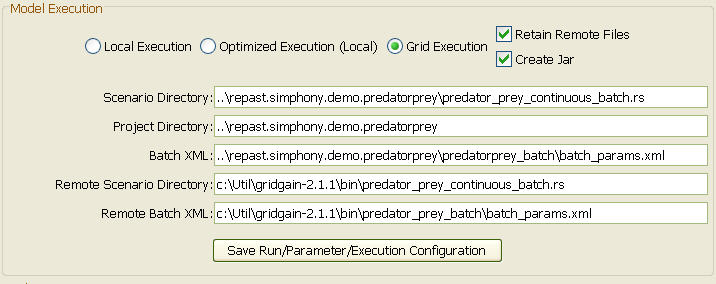
\includegraphics{images/sweep4c.jpg}
}
\caption{}
\label{fig:sweep4c}
\end{center}
\end{figure}

\begin{figure}[h]
\begin{center}
\vspace{.2in}
\centerline {

\includegraphics{images/sweep4d.jpg}
}
\caption{}
\label{fig:sweep4d}
\end{center}
\end{figure}

In addition to the Scenario Directory, the user must specify: the
Project Directory, the batch XML file, the Remote Project Directory,
and the remote Batch XML file (see Fig. ~\ref{fig:sweep4c}). These
items are defined in Section 2. Note that there are two checkboxes activated in Grid Execution mode: Retain Remote Files and Create Jar. The Retain Remote Files checkbox specifies whether or not the model output files will be deleted on the remote GridGain nodes. The Create Jar checkbox specifies whether or not the project jar file will be created for the user. The Save Configuration button can be used to save in the scenario directory a file containing the definitions for all three execution modes that will be loaded during future executions of the scenario.

Finally, Section D (see Fig. ~\ref{fig:sweep5}) contains the button that will submit the job(s) for execution in one of the three modes. Note that the button text will reflect the execution mode that has been selected in Section C.

\begin{figure}[h]
\begin{center}
\vspace{.2in}
\centerline {
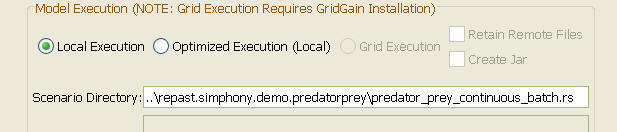
\includegraphics{images/sweep5.jpg}
}
\caption{}
\label{fig:sweep5}
\end{center}
\end{figure}

When the parameter sweep job has been submitted for execution, a console log window will open and display messages from Repast Simphony and/or GridGain depending on the execution type. See  Fig. ~\ref{fig:sweep6} for an example of this window.

\begin{figure}[h]
\begin{center}
\vspace{.2in}
\centerline {
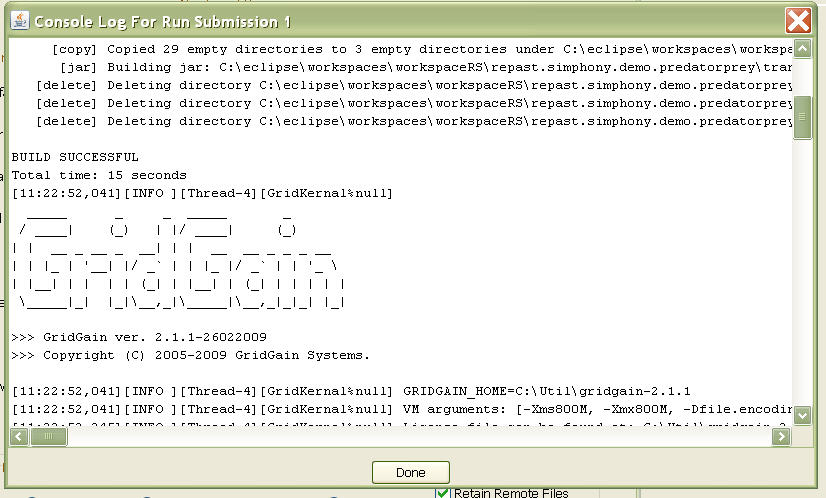
\includegraphics{images/sweep6.jpg}
}
\caption{}
\label{fig:sweep6}
\end{center}
\end{figure}

\section{Developing a Distributed Batch Repast Simphony Project}

A new feature within Repast Simphony is a largely automated distributed batch framework that allows users to distributed their
simulations in batch mode using multiple computer nodes and/or cores. This feature takes advantage of Repast Simphony's previous batch development but adds a new layer of capability in a plugin called repast.simphony.distributedBatch. The instructions below detail how users can setup their own distributed batch process using a Predator Prey project example. Previous Repast capability in allowing users to conduct single node batch runs are still enabled in the 2.0 version of Repast Simphony. This is done, as in previous versions of Repast Simphony, in the repast.simphony.batch plugin.

\subsection{Downloading and Installing GridGain}
The first step in using distributed batch for your project is to go to
the GridGain website (\url{http://www.gridgain.com/}) and download GridgGain 2.1.1 at:\url{http://www.gridgain.com/past_downloads.html}
or at the following
address 
\url{http://mac.softpedia.com/get/Development/Java/Gridgain.shtml}. Repast Simphony is
currently using GridGain 2.1.1 because during the time of development
this was the stable version released by GridGain. In addition, a new
licensing scheme by GridGain makes the 2.1.1. version more feasible
for Repast Simphony than the newer GridGain 3.0 version. For now, the GridGain 2.1.1 version should work well on
Windows (Windows 2000 and up), Mac (Mac OS X versions), and Linux
systems. Users will need to install GirdGain 2.1.1 on all nodes,
including the computer that they are using to launch Repast Simphony
simulations (Fig. ~\ref{fig:g1}). Users should read the GridGain 2.1.1 installation
instructions for proper configuration of GridGain 2.1.1. Once
installed, place the repast.simphony.batch.jar, which is found in
the /transferFiles folder of the repast.simphony.distributedBatch
plugin, into the /libs/ext folder located within the GridGain
installation folder (i.e., [location of the GridGain 2.1.1
folder]/libs/ext) for all nodes that have GridGain installed and those
that will be used for distributed Repast batch runs.

\begin{figure}[h]
\begin{center}
\vspace{.2in}
\centerline {
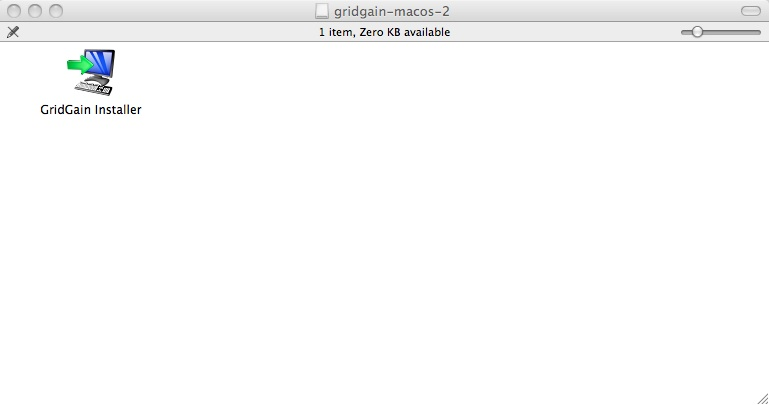
\includegraphics[width=\textwidth]{images/Figure1.jpg}
}
\caption{The GirdGain 2.1.1 installer for Mac OS X.}
\label{fig:g1}
\end{center}
\end{figure}

The default-spring.xml file, found in repast.simphony.distributedBatch, should be used to replace the
default-spring.xml file in the /config folder within the GridGain 2.1.1 installation folder on all nodes used (Fig. ~\ref{fig:g2}). This file will allow the default distributed configuration on all nodes used to be the same as that found in the repast.simphony.distributedBatch folder, which controlles the configuration of the user's computer where processes are launched from.

\begin{figure}[h]
\begin{center}
\vspace{.2in}
\centerline {
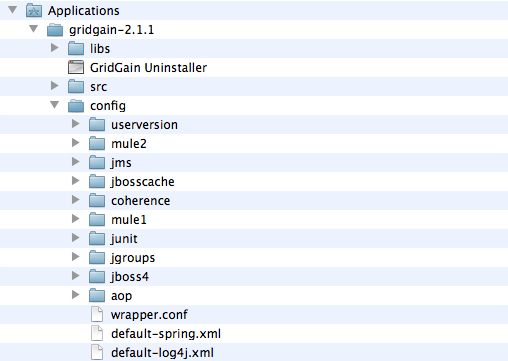
\includegraphics[width=\textwidth]{images/Figure2.jpg}
}
\caption{default-spring.xml file location}
\label{fig:g2}
\end{center}
\end{figure}

The next step is creating a standard batch file, often called
batch\_params.xml, which contains the simulation parameters and number
of batch runs. The documentation above described how to create one using
the batch parameters GUI. You can do that or create one by hand. Because the project is a distributed batch project,
users should set the ``sweep runs'' setting to 1, as the sweep setting
will now be handled by the distributed process. If a user desires to
run a regular batch run (i.e., using only one node), then the user
should set the sweep runs setting to whatever number he or she
desires. (Fig. ~\ref{fig:g3}) below shows what a standard
batch\_params.xml file looks like. This file should be placed
somewhere within the user's Repast project folder. You should also remember to setup outputs as 
you normally would for Repast Simphony projects (e.g., text file outputters).

\begin{figure}[h]
\begin{center}
\vspace{.2in}
\centerline {
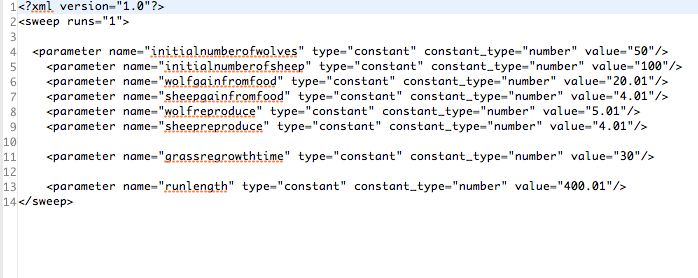
\includegraphics[width=\textwidth]{images/Figure3.jpg}
}
\caption{Example Batch File}
\label{fig:g3}
\end{center}
\end{figure}

\subsection{Creating the Project Jar File}
The user then has two options for creating a project jar file to be
used in the distributed runs. The first option is to use the GUI described above,
and make sure the Create Jar options is selected.

Alternatively, the Eclipse Repast Simphony IDE can be used. In this option, the user needs to
click on their project and create a jar file by choosing File $\rightarrow{}$ Export$ \rightarrow{}$ JAR file.
Then, in the ``Jar Export'' window (Fig. ~\ref{fig:g4}), name the project jar
and export it. The user will then need to place this jar file in the
/transferFiles folder located in their project folder.

\begin{figure}[h]
\begin{center}
\vspace{.2in}
\centerline {
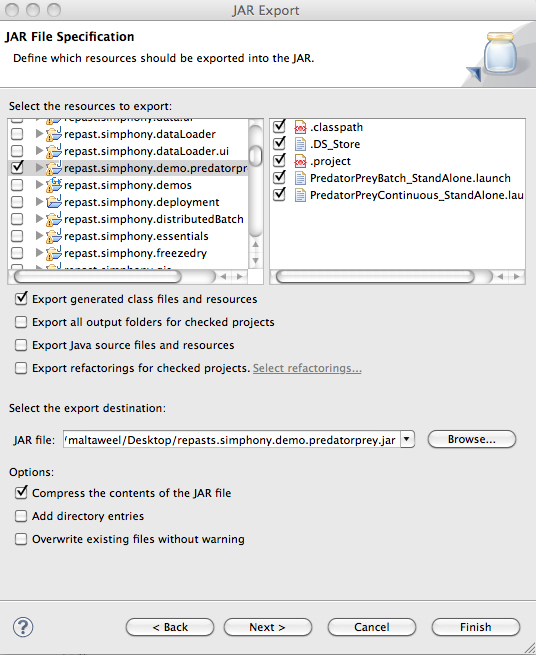
\includegraphics[width=\textwidth]{images/Figure4.jpg}
}
\caption{Jar Exporting}
\label{fig:g4}
\end{center}
\end{figure}

\subsection{Setting the Distributed Batch Runs}


Next, the user sets up a project that uses the repast.simphony.distributedBatch plugin. There are several path settings that need to be determined for both the local node (i.e., the computer you are using to launch the process) and the remote nodes. First, look at the XML\_Launch\_Inputs.xml file located in the /launchData folder within the repast.simphony.distributedBatch plugin. You will need to edit the following sets of paths and data
(Fig. ~\ref{fig:g5} \& Fig. ~\ref{fig:g6}).

\begin{figure}[h]
\begin{center}
\vspace{.2in}
\centerline {
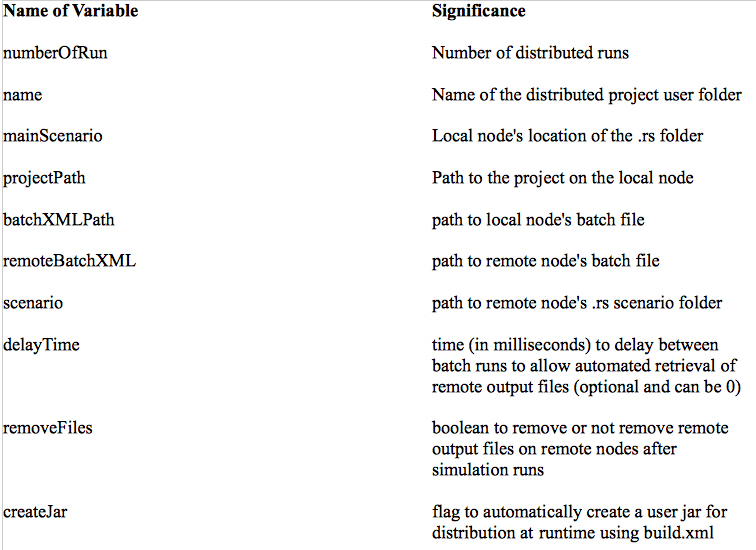
\includegraphics[width=\textwidth]{images/Figure5.jpg}
}
\caption{XML\_Launch\_Inputs.xml file's user inputs}
\label{fig:g5}
\end{center}
\end{figure}

\begin{figure}[h]
\begin{center}
\vspace{.2in}
\centerline {
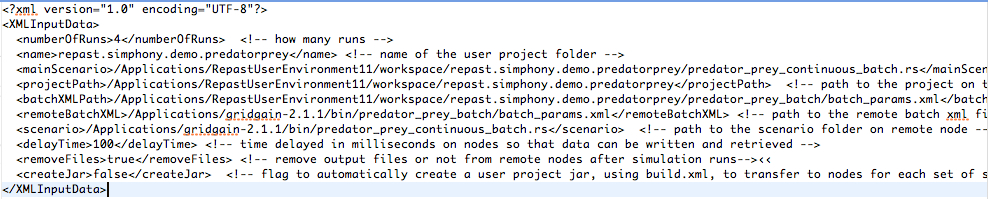
\includegraphics[width=\textwidth]{images/Figure6.jpg}
}
\caption{XML\_Launch\_Inputs.xm}
\label{fig:g6}
\end{center}
\end{figure}

Repast Simphony applies a ``user\_path.xml'' file that is typically
located in the user's .rs folder (see
repast.simphony.demo.predatorprey as an example). This file allows
Repast Simphony to loaded necessary classes for simulation runs and is
used for regular GUI simulations, regular batch simulation, and
distributed batch runs. In addition to setting the local bin folder's
location, the user needs to indicate where the remote nodes' class bin
folder will be located. In the repast.simphony.distributedBatch
plugin, the processes will launch on the remote nodes from GridGain's
installation /bin folder. When a distributed processes is launched,
the user's .jar project file will be unjared, exposing the class files
in the jar file. The class files will be typically located in the
GridGain /bin folder at that point. Thus, users will need to indicate
a path where the users' classes are located in GridGain. Typically,
the user should place a class reference to the GridGain bin folder (Fig. ~\ref{fig:g7}). However, if the jar was created the gui they may need to reference their project's bin folder within the bin
of GridGain (Fig. ~\ref{fig:g8}). The two /bin
  references are needed because the user's jar has its own bin folder.

\begin{figure}[h]
\begin{center}
\vspace{.2in}
\centerline {
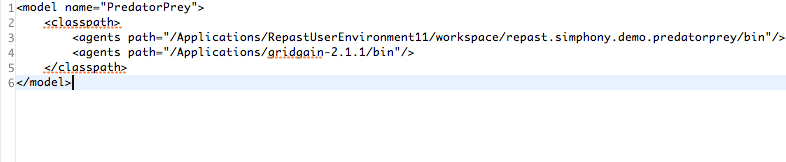
\includegraphics[width=\textwidth]{images/Figure7.jpg}
}
\caption{Remote Bin Folder}
\label{fig:g7}
\end{center}
\end{figure}

\begin{figure}[h]
\begin{center}
\vspace{.2in}
\centerline {
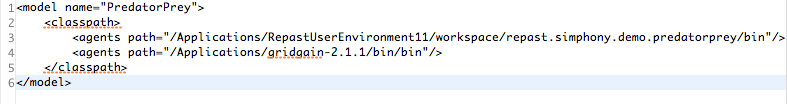
\includegraphics[width=\textwidth]{images/Figure8.jpg}
}
\caption{The reference to the remote
  bin folder seen for projects using ant build.xml file. The two /bin
  references are needed because the user's jar has its own bin folder.
}
\label{fig:g8}
\end{center}
\end{figure}

\subsection{Launching the Remote Nodes}

\begin{figure}[h]
\begin{center}
\vspace{.2in}
\centerline {
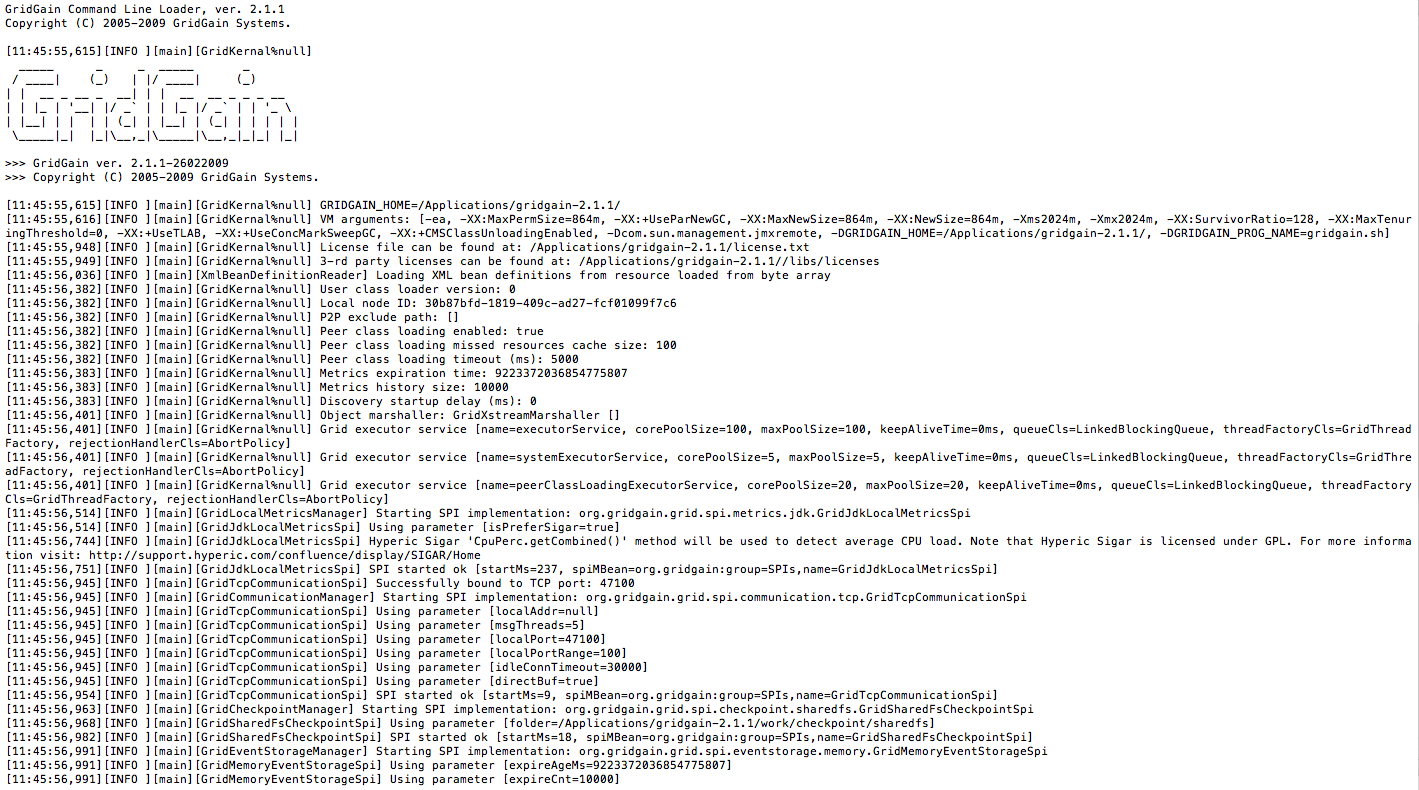
\includegraphics[width=\textwidth]{images/Figure9.jpg}
}
\caption{Launched Remote Node}
\label{fig:g9}
\end{center}
\end{figure}



The user is now ready to launch the remote nodes. First, be sure to
have the JAVA\_HOME and GRIDGAIN\_HOME variables set on the remote
nodes, as stated by the GridGain installation instructions (please
read the GridGain 2.1.1 instructions prior to using GridGain in
Repast). To launch GridGain, simply login into your remote nodes and
launch the ``gridgain.sh'' file or ``gridgain.bat'' file (.sh for Mac and
Linux and .bat for Windows machines). For Mac and Linux machines, type
``sh [path to gridgain.sh file]/gridgain.sh'' in the line command on
the remote node, which should then activae your remote node. For
Windows machines, just type the following path ``[path to gridgain.bat
file]/gridgain.bat'' to do the same process as the other operating
systems. Once launched, you do not need to turn off any nodes if you plan
on running multiple sets of distributed batch runs. However, if any
launch errors occur on the remote nodes or you edit your code, then you will
need to restart the remote nodes as the new classes or updated classes
will need to be reloaded on the remote machines. You may also want to
configure a startup script that will automatically launch your
GridGain startup files on the remote nodes. Once launched, you should
see the remote nodes producing log information that indicates they are
ready to receive processes launched from your local computer and can
connect to other nodes in a cluster  (Fig. ~\ref{fig:g9}).

\subsection{Launching the Distributed Process}

\begin{figure}[h]
\begin{center}
\vspace{.2in}
\centerline {
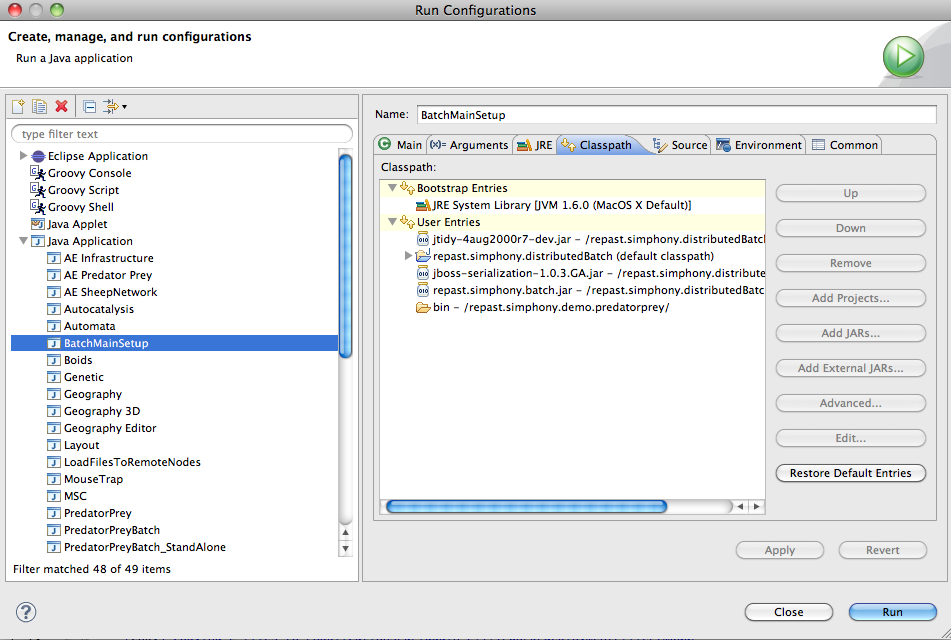
\includegraphics[width=\textwidth]{images/Figure10.jpg}
}
\caption{Reference To the Local Bin Folder}
\label{fig:g10}
\end{center}
\end{figure}

\begin{figure}[h]
\begin{center}
\vspace{.2in}
\centerline {
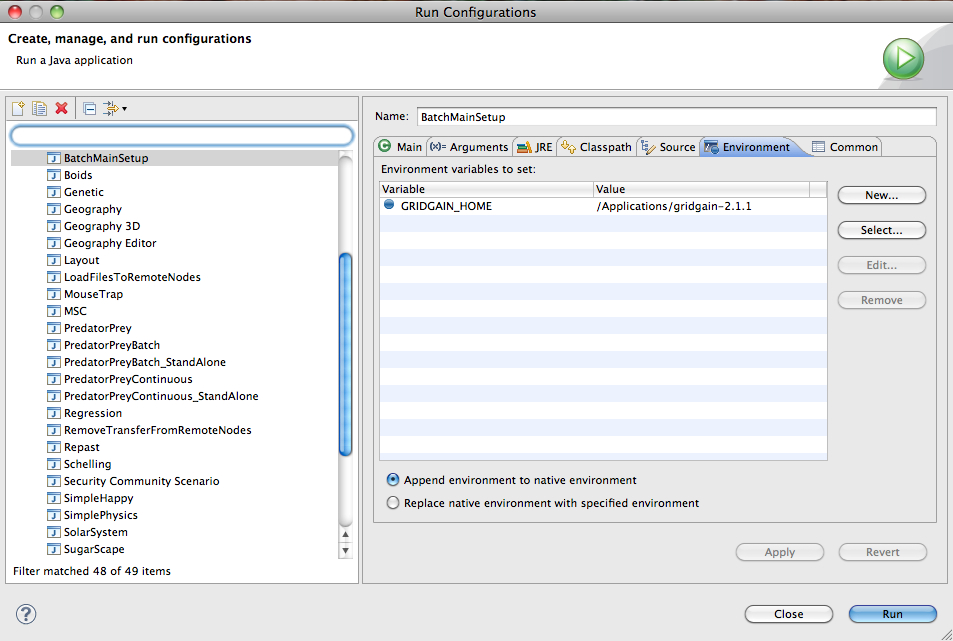
\includegraphics[width=\textwidth]{images/Figure11.jpg}
}
\caption{Environment reference to the GridGain installation folder.}
\label{fig:g11}
\end{center}
\end{figure}


The user can now launch the distributed process. The user can now
revert to using the GUI Parameter Sweep setup (see above) or use a Java
Application launch configuration in Eclipse. To do this second option, go to Run
Configurations... in the Repast Simphony Eclipse IDE and in the
run configurations window select the Java Application setup for
BatchMainSetup. There, choose the Classpath tab in the Run
Configurations window. Add the local user project's bin folder to the
User Entries (Fig. ~\ref{fig:g10}). Then, in the Environment tab edit the local
path to the GRIDGAIN\_HOME�directory of the GridGain installation
folder (Figure 11). This will automatically startup your local GridGain
application at runtime. Users can also create their own Run
Configurations... setup using similar
settings to the ``'BatchMainSetup.launch'' file located in the
Repast Simphony distributedBatch plugin folder. 


\begin{figure}[h]
\begin{center}
\vspace{.2in}
\centerline {
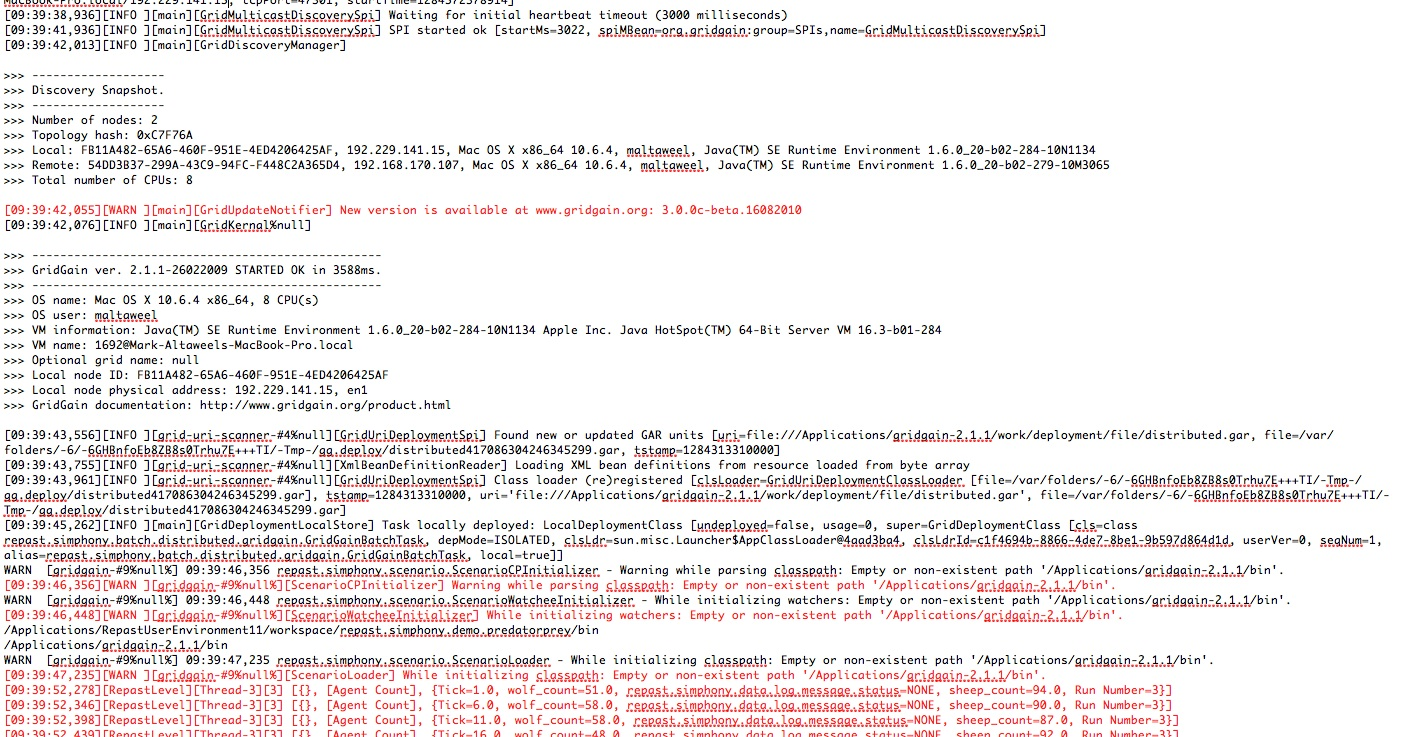
\includegraphics[width=\textwidth]{images/Figure12.jpg}
}
\caption{Local node distributed batch output.}
\label{fig:g12}
\end{center}
\end{figure}

\begin{figure}[h]
\begin{center}
\vspace{.2in}
\centerline {
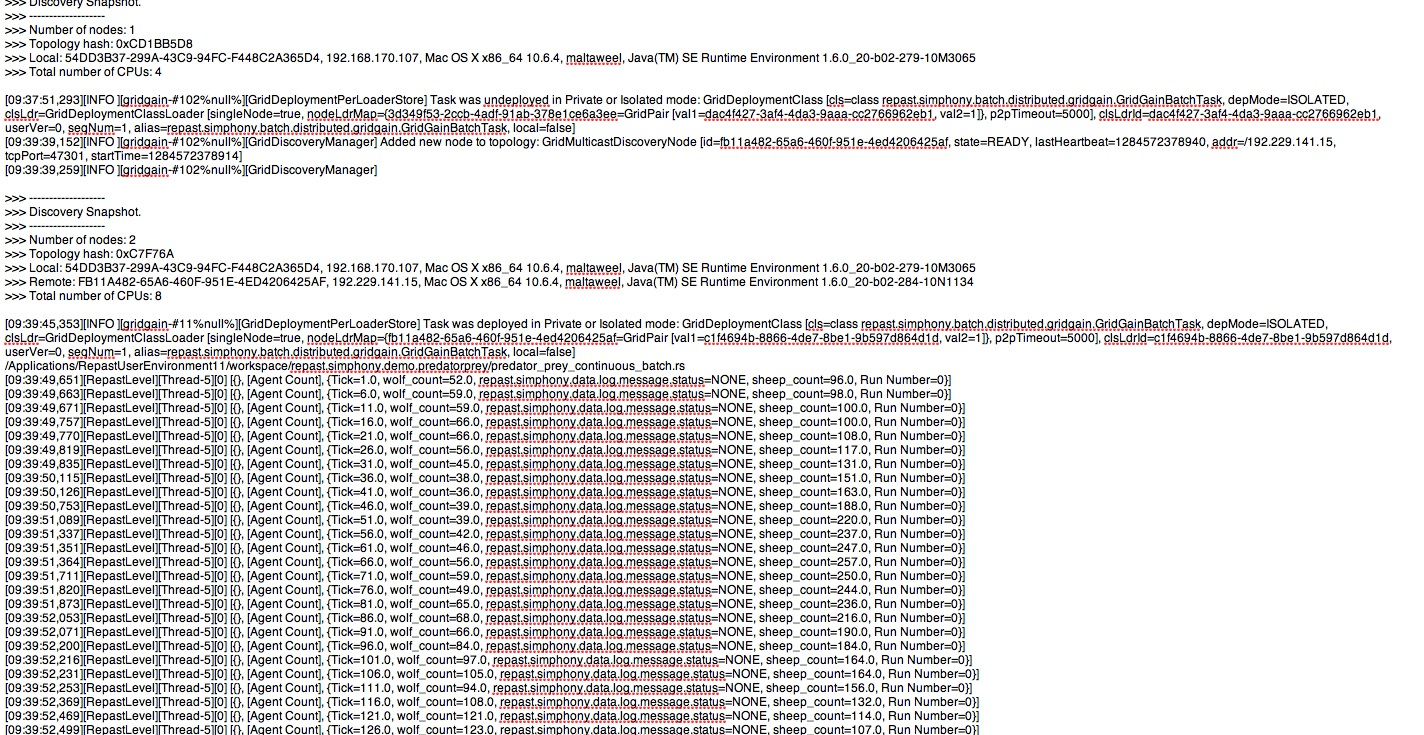
\includegraphics[width=\textwidth]{images/Figure13.jpg}
}
\caption{Remote node distributed batch output.}
\label{fig:g13}
\end{center}
\end{figure}


Now, the user can select the Run button in the Run Configurations
window (bottom right corner in Run Configurations) and launch the distributed process. The
log should produce output information in the local console window
(Fig. ~\ref{fig:g12}) and remote nodes (Fig. ~\ref{fig:g13}), showing the distributed
process running. The output should include information on the number
of nodes running in GridGain and any output console information
produced by the user's project (e.g., in the Predator Prey example the
outputter, setup in the Repast GUI environment, displays user
output). You should also see unique threads running on the local and
remote nodes. The example Predator Prey project ((Fig. ~\ref{fig:g12} and Fig. ~\ref{fig:g13})
shows two nodes (i.e., two computers) executing the model. Another featured in
distributed batch is that it uses automatic failover, which allows
other nodes to take the jobs from machines that may fail during the
batch process. 


\section{Outputs Produced}

Outputs produced by the remote and local nodes will be collected and
placed in the /output folder of the users' project (e.g., see
the /output folder in repast.simphony.demo.predatorprey). The output files should be unique for
each run. Remote nodes' outputs that are transferred to the /output
folder may require that the user set a value for the ``delayTime'' parameter in the
XML\_Launch\_Inputs.xml file to enable output results to be transferred to the local node (i.e., the delay would allow enough
time to create the output file and to be transferred over). The local node
may also write local node results to the distributedBatch plugin
path. The user, if desired, can remove these outputs as they will also
be automatically copied over to the /output folder in their project folder. In addition, remote nodes will create output files in the
/bin directories of the GridGain installation on remote nodes. These files are automatically removed if the user
sets the ``removeFiles'' option in XML\_Launch\_Inputs.xml to
``true''. If the user chooses to remove remote output files, these
files will still be transferred to the /output folder in the user's project.





\end{document}
